% !TeX program = xelatex
\PassOptionsToPackage{quiet}{fontspec}
\documentclass[12pt,a4paper,UTF8]{ctexart}
\usepackage{projectreport}

\projecttitle{SuperKnob 基于 ESP32 的FOC多功能智能旋钮}
\projectcourse{嵌入式系统高级实践}
\projectmembers{李彦霖（组长），朱熠正，康鑫杰}{ }
\projectschool{控制科学与工程学院}
\projectteacher{陆玲霞，叶炜}
\projectdate{2026 年 9 月}

\begin{document}
\makeprojectcover
\setcounter{tocdepth}{2}
\tableofcontents
\newpage

\section*{摘要}
\addcontentsline{toc}{section}{摘要}

SuperKnob 是一套以 ESP32、三相无刷电机、AS5600 磁编码器和 ST7789 显示屏为核心的智能旋钮系统。项目用电机主动输出的可控作用力替代固定机械结构，使同一套硬件能够通过软件切换棘轮、边界、阻尼和弹簧四类触感，并把旋转与触摸输入用于图形界面、电脑控制、计时提醒、音乐演奏、物联网设备控制和小游戏等场景。

系统的软件结构围绕实时控制与图形交互的解耦展开。电机任务固定运行在 ESP32 Core 1，持续读取 AS5600 的角度与速度并执行 SimpleFOC 闭环换相；LVGL 任务固定运行在 Core 0，负责屏幕刷新、页面状态和输入事件。两个任务通过 FreeRTOS 队列传递页面切换、点击反馈、音乐播放和弹簧模式等控制事件，并通过另一条队列返回电机初始化状态。现有代码没有配置相电流采样，因此触感算法给出的“力矩”在实现上是受限的 q 轴电压指令。该实现足以形成稳定可辨识的旋钮触感，同时也明确了后续升级到电流闭环转矩控制的接口边界。

\textbf{关键词：}智能旋钮；磁场定向控制；软件定义触感；FreeRTOS；LVGL；ESP32

\section{项目简介}

\subsection{项目背景与目标}

传统旋钮依靠弹簧、钢珠、限位柱等机械结构形成段落感与边界感。一旦机械结构确定，旋钮的档位数量、档距和回弹方式也随之固定。SuperKnob 将无刷电机作为双向力反馈执行器，把“旋钮应该如何用力”写成可切换的控制规律。页面或功能改变时，系统只需修改目标作用力的计算方式，就能让同一个旋钮表现为有清晰吸附点的菜单滚轮、带上下限的参数旋钮、松手回中的弹簧杆，或仅在运动时产生阻力的连续控制器。

项目的工程目标包括三部分。第一，完成 ESP32、BLDC、磁编码器、显示屏、驱动板和触摸输入的整机集成。第二，在 SimpleFOC 的基础上实现稳定的力反馈控制，并把触感参数封装为可切换配置。第三，以 LVGL 页面、BLE HID、局域网风扇控制、计时器、音乐和游戏验证旋钮交互在不同任务中的适配能力。

\subsection{系统功能与代码范围}

当前固件的主界面包含台灯、番茄钟、音乐、风扇、游戏、跳一跳、电脑、传感器和关于等入口。答辩 PPT 将电脑控制概括为网页滚轮、音量调节和 Alt+Tab 三种模式；现有 \texttt{bluetooth\_mouse.cpp} 还实现了第四种鼠标左右键模式，因此固件通过触摸 GPIO0 实际循环切换四种 PC 子模式。

报告涉及的主要源文件见表 \ref{tab:source-map}。其中，\texttt{motor.cpp} 是 FOC 与触感算法的核心；\texttt{main.cpp}、\texttt{display.cpp} 共同定义双核任务和队列通信；各页面文件负责在具体交互场景中选择触感配置或发送控制事件。

\begin{table}[H]
\centering
\small
\begin{tabular}{p{0.27\linewidth}p{0.60\linewidth}}
\toprule
源文件 & 主要职责 \\
\midrule
\texttt{src/main.cpp} & 创建消息队列，选择主界面或 PC 运行模式，将 LVGL 与 FOC 任务固定到不同 CPU 核 \\
\texttt{src/motor.cpp} & 初始化 AS5600、三相驱动和 SimpleFOC，计算棘轮、边界、阻尼与弹簧触感，处理音乐 PWM \\
\texttt{src/display.cpp} & 初始化 TFT 与 LVGL，读取旋钮位置和触摸输入，收发跨任务消息 \\
\texttt{src/bluetooth\_mouse.cpp} & 将旋钮角度映射为网页滚轮、音量、Alt+Tab 和鼠标左右键输入 \\
\texttt{src/ui\_pages/*.cpp} & 构建功能页面，并根据页面状态切换 KnobConfig 或发送事件 \\
\bottomrule
\end{tabular}
\caption{项目主要代码模块}
\label{tab:source-map}
\end{table}

\subsection{总体工作链路}

图 \ref{fig:system-chain} 表示旋钮的闭环工作链路。AS5600 读取电机轴角度，ESP32 根据页面状态选择触感模型并计算控制量，SimpleFOC 把控制量转换成三相 PWM，电机再把力反馈施加到用户手上。与此同时，LVGL 将同一角度信息解释为菜单焦点变化、参数增减或游戏输入。系统因此形成“物理运动、控制计算、界面状态、触感反馈”相互关联的交互闭环。

\begin{figure}[H]
\centering
\begin{tikzpicture}[
  node distance=1.15cm and 1.0cm,
  box/.style={draw=black!55, rounded corners=2pt, align=center, minimum height=1.05cm, text width=2.55cm, fill=black!2},
  arr/.style={-{Latex[length=2.6mm]}, thick, draw=black!70}
]
\node[box] (user) {用户旋转或触摸};
\node[box, right=of user] (sensor) {AS5600\\角度与速度};
\node[box, right=of sensor] (esp) {ESP32\\触感模型与页面逻辑};
\node[box, right=of esp] (driver) {SimpleFOC 与\\三相 PWM 驱动};
\node[box, below=1.15cm of esp] (motor) {BLDC 输出作用力\\形成触感反馈};
\draw[arr] (user) -- (sensor);
\draw[arr] (sensor) -- (esp);
\draw[arr] (esp) -- (driver);
\draw[arr] (driver) |- (motor);
\draw[arr] (motor) -| node[pos=0.2, below]{机械反馈} (user);
\end{tikzpicture}
\caption{SuperKnob 的输入、控制与反馈链路}
\label{fig:system-chain}
\end{figure}

% 第 2--3 章：硬件平台与软件平台
% 第 2--3 章：硬件平台与软件平台
\section{硬件平台}

\subsection{核心硬件组成}

主控采用 ESP32 LOLIN32 Lite。该芯片提供双核处理器、FreeRTOS 运行环境、I2C、SPI、PWM、Wi-Fi 与 BLE，能够在单芯片上并行承担图形界面、电机控制和无线通信。执行器为 2804 三相无刷电机，代码按 7 对极建立 \texttt{BLDCMotor(7)} 对象。电机由三路 PWM 驱动板控制，使能脚由 GPIO12 管理。转子位置由 AS5600 磁编码器提供，固件以 400 kHz I2C 读取传感器。

显示模块使用 240\,$\times$\,320 分辨率的 ST7789 TFT，TFT\_eSPI 负责 SPI 传输，LVGL 负责页面与控件。显示任务申请一块 240\,$\times$\,40 像素的内部 DMA 缓冲区，约占 19.2 KB，通过分条刷新降低图形缓冲对 ESP32 内存的压力。GPIO0 的电容触摸通道同时承担页面确认以及 PC 模式切换输入。

\begin{table}[H]
\centering
\small
\begin{tabular}{p{0.22\linewidth}p{0.23\linewidth}p{0.43\linewidth}}
\toprule
模块 & 型号或接口 & 在系统中的作用 \\
\midrule
主控 & ESP32 LOLIN32 Lite & 运行 Arduino 框架、FreeRTOS、LVGL、SimpleFOC、Wi-Fi 与 BLE \\
执行器 & 2804 BLDC，7 对极 & 输出双向可控作用力，形成触感与振动反馈 \\
位置反馈 & AS5600，I2C 地址 0x36 & 读取机械角度，供 FOC 和交互逻辑计算位置与速度 \\
电机驱动 & 三相 3PWM 驱动板 & 接收 ESP32 的三路 PWM 并驱动 BLDC，相电源按 12 V 配置 \\
显示 & ST7789，240\,$\times$\,320 & 显示主菜单、状态信息与各功能页面 \\
触摸输入 & ESP32 GPIO0 电容触摸 & 作为确认、退出及 PC 子模式切换按键 \\
结构件 & 自研转接板与外壳 & 组织屏幕、主控、驱动、编码器及电机的电气和机械连接 \\
\bottomrule
\end{tabular}
\caption{SuperKnob 核心硬件}
\label{tab:hardware}
\end{table}

\subsection{关键接口与引脚}

表 \ref{tab:pins} 汇总了 \texttt{motor.cpp} 与 \texttt{platformio.ini} 中的实际引脚配置。电机与屏幕分别占用不同的 PWM、I2C 和 SPI 资源，便于在双核任务中并行运行。电机驱动的 \texttt{voltage\_power\_supply} 设置为 12 V，固件把控制电压上限设为 8 V；初始化时还通过 1000 个递增步骤逐渐放开电压限幅，以减轻对齐完成后的突发作用力。

\begin{table}[H]
\centering
\small
\begin{tabular}{p{0.29\linewidth}p{0.21\linewidth}p{0.37\linewidth}}
\toprule
信号 & ESP32 引脚 & 说明 \\
\midrule
电机 PWM A/B/C & 32 / 33 / 25 & 三相 3PWM 输出 \\
电机使能 & 12 & 高电平使能驱动板 \\
AS5600 SDA/SCL & 23 / 5 & 400 kHz I2C 总线 \\
TFT MOSI/SCLK & 19 / 18 & ST7789 SPI 数据与时钟 \\
TFT CS/DC/RST/BL & 16 / 15 / 13 / 17 & 片选、数据命令、复位与背光 \\
触摸确认 & 0 & 电容触摸通道 \\
\bottomrule
\end{tabular}
\caption{固件中的关键引脚配置}
\label{tab:pins}
\end{table}

\subsection{信号闭环与结构集成}

磁铁与电机轴同轴安装后，AS5600 提供连续机械角度。ESP32 将机械角与 7 对极相乘得到电角度，并根据初始化得到的零电角完成换相。三相驱动板把 PWM 占空比转换为绕组电压，电机产生的反作用力通过旋钮轴直接反馈给用户。屏幕、编码器、电机驱动和主控之间的连接由自研转接板重新组织，外壳则负责保证磁铁、编码器、电机轴和显示屏的相对位置。该结构要求电气闭环和机械同轴度同时满足条件，任何安装偏心、磁铁距离不合适或供电压降都会直接表现为触感波动。

\section{软件平台}

\subsection{开发环境与依赖}

工程使用 PlatformIO 管理构建和依赖，目标环境为 \texttt{lolin32\_lite}，底层采用 Arduino framework。\texttt{platformio.ini} 固定了主要库版本与 TFT 配置，表 \ref{tab:software-stack} 列出实际软件栈。项目同时内置 BleCombo 源码，用同一 BLE 连接提供键盘和鼠标 HID 能力。

\begin{table}[H]
\centering
\small
\begin{tabular}{p{0.28\linewidth}p{0.22\linewidth}p{0.38\linewidth}}
\toprule
组件 & 版本或配置 & 用途 \\
\midrule
PlatformIO Espressif32 & 7.1.1 & 工程构建、下载与依赖管理 \\
Arduino framework & ESP32 平台默认版本 & 硬件接口、任务入口与兼容库运行环境 \\
SimpleFOC & 2.2.1 & 传感器角度接入、FOC 换相和 3PWM 输出 \\
LVGL & 8.4.0 & 页面、控件、动画、输入设备与定时器 \\
TFT\_eSPI & 2.5.0 & ST7789 SPI 显示驱动与 DMA 刷新 \\
ESP32 BLE Keyboard & 0.3.2 兼容版本 & BLE HID 键盘基础能力 \\
项目内置 BleCombo & 本地源码 & 组合键盘与鼠标 HID \\
\bottomrule
\end{tabular}
\caption{项目软件栈}
\label{tab:software-stack}
\end{table}

\subsection{软件分层}

应用层由各 LVGL 页面和功能控制器组成。页面通过旋转和触摸完成焦点切换、参数调节与状态显示。交互层位于 \texttt{display.cpp}，将电机配置中的离散位置变化转换为 LVGL 的 \texttt{enc\_diff}，并对 GPIO0 触摸进行连续采样和锁存消抖。任务与通信层由 FreeRTOS 任务、队列、软件定时器以及少量临界区构成。控制层位于 \texttt{motor.cpp}，负责角度采样、FOC 更新和触感控制量计算。驱动层包括 SimpleFOC、TFT\_eSPI、BleCombo、Wi-Fi UDP 与 ESP32 LEDC。

这种分层使页面不直接操作三相 PWM。页面只选择 \texttt{KnobConfig} 或发送事件，电机任务在自己的循环中执行配置更新。钓鱼游戏选择配置 5 进入纯粘性阻尼，跳一跳发送 \texttt{JUMP\_SPRING\_START} 进入独立弹簧状态机，音乐页面发送 \texttt{MUSIC\_PLAY} 暂时把三路 PWM 资源切换到 LEDC 音符输出。

\subsection{两种启动模式}

固件通过 RTC 非初始化内存中的 \texttt{current\_os\_mode} 区分主界面模式与 PC 模式。硬件复位时该变量被强制置零，系统创建 LVGL 任务并启动主界面；软件重启进入 PC 模式时保留该变量，只直接初始化 TFT 并启动 BLE，从而把较多内存留给 BLE 协议栈。FOC 任务在两种模式中都会启动。PC 模式下，电机任务直接调用 \texttt{run\_pc\_mouse\_logic()}，根据旋钮角度同时生成 HID 事件和对应作用力。


% 第 4--6 章：FOC、四种手感与 FreeRTOS 双核通信
% 第 4--6 章：FOC、四种手感与 FreeRTOS 双核通信
\section{FOC 原理及其在项目中的应用}

\subsection{磁场定向控制的基本思想}

三相无刷电机需要按照转子磁场方向切换定子电压。FOC 将三相静止坐标系中的电气量变换到随转子旋转的 $d$-$q$ 坐标系，使励磁方向与产生转矩的方向相互正交。以两相静止坐标为中间量，典型 Park 变换可写为

\begin{equation}
\begin{bmatrix}x_d\\x_q\end{bmatrix}
=
\begin{bmatrix}
\cos\theta_e & \sin\theta_e\\
-\sin\theta_e & \cos\theta_e
\end{bmatrix}
\begin{bmatrix}x_\alpha\\x_\beta\end{bmatrix},
\end{equation}

其中 $\theta_e$ 是电角度。对于 7 对极电机，电角度在忽略零点偏置时满足 $\theta_e=7\theta_m$，$\theta_m$ 为 AS5600 读取的机械角。控制器通常把 $d$ 轴指令设为零，把 $q$ 轴作为主要转矩方向，再通过逆 Park 变换和空间矢量 PWM 生成三相占空比。这样可以避免简单六步换相带来的明显转矩脉动，使旋钮在低速和静止附近也能输出方向连续的作用力。

\subsection{本项目中的控制链路}

本项目把 SimpleFOC 作为“触感执行层”。上层触感算法根据角度误差、角速度、页面边界或游戏状态计算控制量 $u_h$，SimpleFOC 则根据当前电角度把 $u_h$ 施加到合适的 $q$ 轴方向，并用 Space Vector PWM 驱动三相桥。控制链路可表示为图 \ref{fig:foc-chain}。

\begin{figure}[H]
\centering
\begin{tikzpicture}[
  node distance=0.9cm,
  box/.style={draw=black!55, rounded corners=2pt, align=center, minimum height=0.95cm, text width=2.35cm, fill=black!2},
  arr/.style={-{Latex[length=2.4mm]}, thick, draw=black!70}
]
\node[box] (sensor) {AS5600\\机械角 $\theta_m$};
\node[box, right=of sensor] (angle) {极对数与零点\\电角度 $\theta_e$};
\node[box, right=of angle] (law) {触感规律\\生成 $u_h$};
\node[box, right=of law] (foc) {逆变换与 SVPWM\\三相占空比};
\node[box, right=of foc] (plant) {驱动板与 BLDC\\轴上作用力};
\draw[arr] (sensor) -- (angle);
\draw[arr] (angle) -- (law);
\draw[arr] (law) -- (foc);
\draw[arr] (foc) -- (plant);
\draw[arr] (plant.south) |- ++(0,-0.65) -| node[pos=0.25, below]{角度反馈} (sensor.south);
\end{tikzpicture}
\caption{FOC 在 SuperKnob 中的执行链路}
\label{fig:foc-chain}
\end{figure}

代码首先在 23/5 引脚上启动 400 kHz I2C，将 AS5600 连接到电机对象；随后设置驱动电源为 12 V、传感器对齐电压为 3 V，并选择 Space Vector PWM。电机初始化与 FOC 对齐完成后，控制模式从角度控制切换为 \texttt{MotionControlType::torque}。FOC 任务在循环中持续调用 \texttt{motor.loopFOC()}，再调用 \texttt{motor.move(control)} 写入本次触感控制量。

\begin{lstlisting}[caption={FOC 初始化的核心代码结构},label={lst:foc-init}]
I2Cone.begin(23, 5, 400000UL);
sensor.init(&I2Cone);
motor.linkSensor(&sensor);

driver.voltage_power_supply = 12;
driver.init();
motor.linkDriver(&driver);

motor.voltage_sensor_align = 3;
motor.foc_modulation = FOCModulationType::SpaceVectorPWM;
motor.init();
motor.initFOC();

motor.controller = MotionControlType::torque;
motor.loopFOC();
motor.move(control_value);
\end{lstlisting}

\subsection{初始化与运行参数}

初始化阶段使用速度 PID 参数 $P=0.08$、$I=4$、$D=0.0002$，速度低通时间常数为 0.02 s，角度环比例系数为 20，速度上限为 5 rad/s。完成对齐后，\texttt{init\_angle()} 在保持当前角度的同时把控制电压限幅从零逐步提升至 8 V。进入触感循环后，速度 PID 对象被复用于位置误差到控制量的映射：不同档距会改变微分项，不同吸附强度会改变比例项与限幅。

电机任务每轮末尾执行 \texttt{vTaskDelay(1)}。它没有建立固定周期的硬实时定时器，因此实际更新间隔会受 FreeRTOS tick、串口打印和分支路径影响。对当前交互频率而言，该循环足以提供连续触感；若后续需要可量化的带宽与稳定裕度，应使用固定周期调度并记录实际采样间隔。

\subsection{“力矩模式”的实现边界}

项目代码没有创建或链接相电流传感器，也没有设置电流控制器。因此，SimpleFOC 的 torque 模式在当前工程中采用电压型控制：\texttt{motor.move()} 的数值本质上是受 \texttt{voltage\_limit} 约束的 q 轴电压指令，而不是以 N$\cdot$m 为单位的闭环转矩设定值。在电机参数、母线电压和转速变化不大时，q 轴电压与输出作用力近似单调相关，适合通过实验调出清晰触感；但负载、绕组温升和反电动势会改变相同指令对应的真实转矩。

这一边界不影响软件定义触感的结构。触感算法仍然产生带方向和幅值的控制量，FOC 仍然负责按转子方向平滑换相。后续若增加低侧电流采样，只需把底层升级为电流闭环，再重新标定各触感增益，就能提高不同工作条件下的力矩一致性。

\section{四种手感的实现}

\subsection{统一配置结构}

常规触感由 \texttt{KnobConfig} 描述，字段包括位置数量、当前位置、单格角宽、吸附强度、边界强度、跨格阈值和阻尼强度。页面通过 \texttt{update\_motor\_config(index)} 复制预设配置，随后发送 \texttt{CHECKOUT\_PAGE}，电机任务将当前轴角设置为新的吸附中心并刷新控制参数。该机制把“页面选择何种触感”和“电机如何连续计算作用力”分离开来。

\subsection{棘轮触感}

棘轮模式维护当前吸附中心 $\theta_c$。轴角与中心的偏差为
\begin{equation}
e_\theta=\theta_m-\theta_c.
\end{equation}
当 $e_\theta$ 超过“档距 $\times$ 跨格阈值”时，程序把 $\theta_c$ 平移一个档距，并同步增加或减少逻辑位置。未跨格时，控制器持续把旋钮拉回最近吸附中心。中心附近设置一个不超过 1$^\circ$ 的死区，减小静止抖动；旋钮静止 500 ms 且仍位于中心附近时，中心以很小的系数缓慢跟随实测角度，用于消除长期偏置。

主菜单使用配置 1：档距约 8.226$^\circ$，吸附强度 2.3，位置数量为 0 表示不限制档位数。风扇详情页沿用同一物理档距和强度，在页面软件侧把输入灵敏度放大 2 倍，避免通过缩小闭环档距来牺牲稳定性。

\subsection{边界触感}

边界模式在有限位置范围的首端或末端检测越界方向。如果用户继续向范围外旋转，程序把速度 PID 的比例系数从吸附强度对应值切换为边界强度对应值，同时把输出限幅从 3 提高到 10，从而产生明显的反向作用力。配置 2 和配置 3 都定义了 256 个位置、1$^\circ$ 档距和起始位置 127；前者带吸附档位，后者关闭档位但保留边界。配置 4 则定义两个相隔 60$^\circ$ 的位置，形成开关式触感。

边界力不是独立的机械挡块，而是有限位置状态与增强控制增益共同形成的软件限位。断电时该限位消失，因此它适合交互提示和参数保护，不应承担人身或结构安全限位功能。

\subsection{阻尼触感}

阻尼模式不设置目标位置，只对转速施加反向控制量：
\begin{equation}
u_h=-b\,\hat{\omega}.
\end{equation}
其中 $b=0.6$，$\hat{\omega}$ 是低通后的轴速度。代码采用指数滑动平均
\begin{equation}
\hat{\omega}_k=(1-\alpha)\hat{\omega}_{k-1}+\alpha\omega_k,
\qquad \alpha=0.05,
\end{equation}
并在 $|\hat{\omega}|\leq0.15$ rad/s 时输出零，超过死区后把控制量限制在 $\pm3$。低通与死区用于抑制 AS5600 量化差分造成的速度尖峰。该模式只有速度项，没有位置恢复项，因此旋转时感觉“发沉”，松手后停在当前位置而不会回到初始点。钓鱼游戏在进入实际游戏阶段时选择配置 5 使用该手感。

\subsection{弹簧触感}

跳一跳采用独立工作模式而不是普通 \texttt{KnobConfig}。进入游戏时，FOC 任务记录中心角 $\theta_0$，令 $\Delta\theta=\theta_m-\theta_0$，并计算
\begin{equation}
u_h=-k\Delta\theta-b\omega,
\qquad k=3.2,\quad b=0.08.
\end{equation}
控制量限制在 $\pm5.5$。当旋转角超过 100$^\circ$ 时，程序叠加额外反向项，使末端逐渐变硬。蓄力比例由 $|\Delta\theta|/100^\circ$ 限制到 0--1 得到。峰值达到 8$^\circ$ 后，如果角度从峰值回落至少 3$^\circ$ 且速度方向指向中心，FOC 任务就把一次“释放”事件写入共享状态，LVGL 游戏任务读取蓄力比例并开始跳跃动画。

PC 模式中的 Alt+Tab 也采用回中型控制，但实现更简化：控制量为 $u_h=-12\Delta\theta$，越过约 0.55 rad 后触发窗口切换，回到 0.5 rad 内释放 Alt 键。另一个鼠标左右键模式使用 $u_h=-15\Delta\theta$，向两侧越过阈值分别按下左右键。

\subsection{触感配置与应用映射}

\begin{table}[H]
\centering
\small
\begin{tabular}{p{0.08\linewidth}p{0.18\linewidth}p{0.17\linewidth}p{0.18\linewidth}p{0.27\linewidth}}
\toprule
索引 & 位置范围 & 档距 & 主要参数 & 代码中的用途 \\
\midrule
0 & 无限制 & 10$^\circ$ & 无吸附 & 进入 PC 系统前的过渡配置 \\
1 & 无限制 & 8.226$^\circ$ & 吸附强度 2.3 & 主菜单、游戏菜单、风扇菜单 \\
2 & 256 档 & 1$^\circ$ & 吸附 1，边界 1 & 台灯、番茄钟等精细离散调节 \\
3 & 256 档 & 1$^\circ$ & 无吸附，边界 1 & 有限范围的连续调节预设 \\
4 & 2 档 & 60$^\circ$ & 跨格阈值 0.55 & 开关式强段落预设 \\
5 & 无限制 & 不适用 & 阻尼 0.6 & 钓鱼游戏的连续追踪 \\
6 & 无限制 & 8.226$^\circ$ & 吸附 2.3 & 风扇详情页，软件侧 2 倍灵敏度 \\
\bottomrule
\end{tabular}
\caption{\texttt{super\_knob\_configs} 预设与应用关系}
\label{tab:haptic-configs}
\end{table}

\section{FreeRTOS 双核调度与跨核通信}

\subsection{任务划分}

主界面模式创建两个固定核任务。\texttt{Task\_lvgl} 的栈大小为 4096 字节、优先级为 3，固定运行在 Core 0；\texttt{Task\_foc} 的栈大小同为 4096 字节、优先级为 2，固定运行在 Core 1。Arduino \texttt{loop()} 只每 10 s 延时一次，不承担实时业务。页面刷新、动画、输入设备和开机进度均在 LVGL 任务中处理；传感器读取、\texttt{loopFOC()}、触感状态机和电机 PWM 更新均在 FOC 任务中处理。

PC 模式为了给 BLE 栈保留内存，不创建 LVGL 任务，只直接在 TFT 上显示模式说明。FOC 任务仍在 Core 1 运行，并在每个循环中执行 BLE HID 角度映射。由此可见，“双核 LVGL + FOC”是主界面模式的结构，PC 模式则退化为电机任务主导的单业务核结构。

\begin{lstlisting}[basicstyle=\ttfamily\footnotesize,caption={任务与队列创建的核心结构},label={lst:task-create}]
motor_msg_Queue = xQueueCreate(10, sizeof(struct _knob_message *));
motor_rcv_Queue = xQueueCreate(10, sizeof(struct _knob_message *));

xTaskCreatePinnedToCore(Task_lvgl, "Task_lvgl", 4096, NULL, 3,
                        &Task_lvgl_Handle, 0);
xTaskCreatePinnedToCore(Task_foc, "Task_foc", 4096, NULL, 2,
                        &Task_foc_Handle, 1);
\end{lstlisting}

\subsection{双向消息队列}

系统创建两条长度为 10 的队列，队列元素均为 \texttt{\_knob\_message*} 指针。\texttt{motor\_rcv\_Queue} 从 UI 指向电机，传递页面或功能事件；\texttt{motor\_msg\_Queue} 从电机指向 UI，传递初始化状态。表 \ref{tab:queue-protocol} 给出了代码中已定义的消息协议。

\begin{table}[H]
\centering
\small
\begin{tabular}{p{0.18\linewidth}p{0.31\linewidth}p{0.39\linewidth}}
\toprule
方向 & 消息 & 电机或界面侧处理 \\
\midrule
UI 到 Motor & \texttt{CHECKOUT\_PAGE} & 以当前轴角重置吸附中心，更新触感参数并产生短振动 \\
UI 到 Motor & \texttt{BUTTON\_CLICK} & 执行正负方向各 2 个短周期的点击振动 \\
UI 到 Motor & \texttt{MUSIC\_PLAY} & 退出常规触感，重配三路 LEDC 并开始播放旋律 \\
UI 到 Motor & \texttt{MUSIC\_STOP} & 停止音乐并通过重启恢复 FOC PWM 资源 \\
UI 到 Motor & \texttt{JUMP\_SPRING\_START} & 记录当前中心角，清空蓄力与释放状态，进入弹簧模式 \\
Motor 到 UI & \texttt{MOTOR\_INIT} & 将开机进度条更新到 30\% \\
Motor 到 UI & \texttt{MOTOR\_INIT\_SUCCESS} & FOC 对齐完成后将进度条更新到 75\% \\
Motor 到 UI & \texttt{MOTOR\_INIT\_END} & 电压渐入完成后更新到 100\%，随后进入主界面 \\
Motor 到 UI & \texttt{MOTOR\_MUSIC\_END} & 界面保留对应处理分支，当前音乐流程实际通过重启返回 \\
\bottomrule
\end{tabular}
\caption{双向队列消息协议}
\label{tab:queue-protocol}
\end{table}

\subsection{页面切换的跨核过程}

以从主菜单进入台灯页面为例，LVGL 的点击回调先创建目标页面并执行切屏动画，再调用 \texttt{update\_motor\_config(2)} 选择 1$^\circ$ 精细档位，最后调用 \texttt{update\_page\_status(CHECKOUT\_PAGE)}。该函数把消息指针压入 \texttt{motor\_rcv\_Queue}。Core 1 上的 FOC 任务以非阻塞方式接收消息，收到后把当前 \texttt{shaft\_angle} 设为新的档位中心，按新配置计算 PID 参数，并执行一次短振动。消息处理结束后，FOC 任务立即回到连续 \texttt{loopFOC()} 循环。

电机初始化状态沿反方向传递。FOC 任务在传感器初始化前、\texttt{initFOC()} 完成后以及电压渐入完成后分别发送三个状态。LVGL 任务最多等待 1 tick 接收消息，并据此更新欢迎页进度条。这样界面不需要轮询底层初始化细节，电机任务也不需要直接访问 LVGL 控件。

\begin{figure}[H]
\centering
\begin{tikzpicture}[
  box/.style={draw=black!55, rounded corners=2pt, align=left, text width=4.6cm, minimum height=1.2cm, fill=black!2, inner sep=8pt},
  arr/.style={-{Latex[length=2.5mm]}, thick, draw=black!70}
]
\node[box] (lvgl) {\textbf{Core 0：Task\_lvgl}\newline TFT 刷新、LVGL 动画、编码器输入、触摸消抖、页面状态};
\node[box, right=3.0cm of lvgl] (foc) {\textbf{Core 1：Task\_foc}\newline AS5600 采样、loopFOC、触感控制、音乐与弹簧状态机};
\draw[arr] ([yshift=7pt]lvgl.east) -- node[above, align=center, font=\scriptsize, fill=white, inner sep=1pt]{motor\_rcv\_Queue\\UI 事件} ([yshift=7pt]foc.west);
\draw[arr] ([yshift=-13pt]foc.west) -- node[below, align=center, font=\scriptsize, fill=white, inner sep=1pt]{motor\_msg\_Queue\\电机状态} ([yshift=-13pt]lvgl.east);
\end{tikzpicture}
\caption{主界面模式下的双核任务与队列}
\label{fig:dual-core}
\end{figure}

\subsection{共享状态与并发保护}

跳一跳的蓄力比例和释放事件没有放入通用队列，而是由 FOC 任务写入三个共享变量，LVGL 任务通过 \texttt{get\_jump\_charge\_percent()} 和 \texttt{consume\_jump\_release()} 读取。代码使用 ESP32 的 \texttt{portMUX\_TYPE} 临界区保护这些变量，避免浮点值或标志在跨核读写时出现不一致。

通用消息队列传递的是指向全局 \texttt{LVGL\_MSG} 与 \texttt{MOTOR\_MSG} 的指针，而不是消息结构体副本。当前事件频率较低，发送后通常会很快被另一核取走；但如果同一方向连续发送多个事件，后一次写入可能在前一次消费前覆盖全局对象。更稳健的实现可以把队列元素大小改为 \texttt{sizeof(\_knob\_message)} 并发送结构体值，或为每条消息使用独立存储。两处 \texttt{xQueueSend} 的等待时间均为 0，队列满时消息会直接丢失，因此后续还应检查返回值并记录溢出。

\subsection{双核设计的收益}

FOC 控制对更新连续性敏感，TFT 刷新和页面动画则可能一次传输较多像素。将两者固定到不同 CPU 核后，显示操作不会直接占用电机任务的执行上下文。队列只传递离散事件与少量状态，页面无需了解 FOC 内部变量，电机任务也无需操作 LVGL 对象。该结构降低了模块耦合，并为局域网控制、BLE 和游戏逻辑继续扩展保留了清晰边界。


% 第 7 章：功能模块
% 第 7 章：功能模块
\section{功能模块}

\subsection{主界面交互}

\subsubsection{从电机角度到界面焦点}

主界面的关键不是单独实现一套滚动算法，而是把电机形成的物理档位直接解释为 LVGL 的焦点移动。FOC 任务持续读取轴角 $\theta_m$，并维护当前档位中心 $\theta_c$。主界面采用配置 1，档距约为 $8.23^\circ$，档位数量设为 0，表示菜单可以连续滚动而不设置机械意义上的首尾限位。当角度偏差
\begin{equation}
e_\theta=\theta_m-\theta_c
\end{equation}
超过档距与跨格阈值的乘积时，电机任务将 $\theta_c$ 平移一个档距，同时把逻辑位置变量 \texttt{position} 加一或减一。这样，连续角度先被触感状态机量化为稳定的整数档位；手停在吸附点附近时，位置值不会因传感器细小波动反复变化。

显示任务把旋钮注册为 \texttt{LV\_INDEV\_TYPE\_ENCODER}。输入回调 \texttt{encoder\_read()} 比较本次与上次的档位值：位置增大时输出 \texttt{enc\_diff=+1}，位置减小时输出 \texttt{enc\_diff=-1}。编码器输入与默认 \texttt{lv\_group} 绑定后，LVGL 按差分方向把焦点移动到前一个或后一个可交互按钮。因此，菜单选择形成了“轴角跨过档位阈值—档位整数变化—编码器差分—焦点切换”的逐级映射。第 6 章已经说明了 FOC 与 LVGL 分核运行及消息传递，本节关注的是这条映射如何把物理旋转转化为用户可见的选择结果。

\subsubsection{焦点的视觉表达与确认操作}

菜单容器使用纵向 Flex 布局，并开启纵向滚动和中心吸附。焦点变化后，目标按钮自动滚动到圆屏中央。为了让列表与圆形屏幕匹配，\texttt{scroll\_event\_cb()} 根据子项中心与容器中心的纵向距离 $d_y$ 计算横向偏移
\begin{equation}
x=r-\sqrt{r^2-d_y^2},\qquad |d_y|<r,
\end{equation}
超出半径时则把 $x$ 限制为 $r$。离中心越远的条目横向缩进越大、透明度越低，于是列表在视觉上呈现沿圆弧远离观察者的效果；位于中心的条目偏移最小且完全不透明，自然成为当前焦点。界面没有额外绘制固定光标，焦点位置、中心吸附和电机档位三者共同给出选择反馈。

GPIO0 的触摸输入在连续检测到有效触摸后向 LVGL 报告按下状态，当前焦点按钮随后产生 \texttt{LV\_EVENT\_CLICKED}。按钮回调负责创建目标页面、播放切屏动画，并按功能需要切换电机配置或工作模式。例如进入番茄钟时换为精细档位，进入音乐时发送播放事件，进入跳一跳时由游戏页面启动弹簧模式。旋转负责“选择”，按下负责“确认”，而每跨一格都能感到真实吸附，使视觉焦点与手上感知保持一致。

\subsection{物联网风扇控制}

\subsubsection{方案选择与通信实现}

这一模块控制的实机型号为 \texttt{xiaomi.fan.p69}。开始时我们考虑过米家云端、Home Assistant 中转和局域网直连三种方案。前两种方案分别需要处理账号登录或依赖一台常开的电脑，因此最后选择让 ESP32 通过家庭 Wi-Fi 直接与风扇通信。这样演示时只要旋钮和风扇处在同一网络中，就能独立完成控制。

米家风扇并不能直接接收普通字符串指令，所以我们在 \texttt{miio\_transport.cpp} 中补写了 miIO 通信过程，包括发现设备、整理请求内容、加密发送以及解析回复；在 \texttt{xiaomi\_fan\_p69.cpp} 中再把“读取状态、开关、调速、左转、右转”等操作封装成简单函数，供上层页面调用。最初参考资料给出的型号是 \texttt{p70}，但实机通信返回的是 \texttt{p69}。我们先用只读请求逐项核对电源、模式、风速和摆风状态，确认属性编号后才加入控制指令，避免因型号判断错误而反复修改界面代码。

\subsubsection{旋钮交互与实际调试}

风扇页面分为开关、风速和左右转动三个功能。旋转旋钮用于调节，触摸用于确认或返回；风速页用刻度盘和指针显示 $1\sim100$ 的数值，左右转动页则用圆弧表示操作方向。页面初版出现过中文字形缺失的问题，后来根据界面实际使用的文字重新生成字库，才保证了圆屏上的显示效果。

实机测试时还发现，如果每转过一格就立即等待风扇回复，画面会有明显停顿。为此我们把联网控制放到单独任务中：界面只记录用户最后调到的风速，网络任务按一定间隔发送；快速连续转动时，中间的旧数值会被新数值替代。左右转动指令也限制发送速度和累计数量，避免旋钮转得太快时风扇在随后很长一段时间内继续动作。这样处理后，电机手感和页面刷新不再被网络等待打断。

风速和转向页面都采用可连续旋转的齿轮手感，旋钮本身不设置硬限位，数值到达边界后由程序限制。每跨过一个档位，界面数值改变 2，既保留了清晰的档位感，也减少了从最低档调到最高档所需的圈数。目前实机已经完成状态读取、开关、风速和页面操作测试；左右转动指令已经能够发出，但单次动作对应的实际角度仍需继续根据风扇表现调整。

\subsection{番茄钟与音乐演奏}

\subsubsection{番茄钟的设计思路与核心功能}

番茄钟把计时与触觉提醒分开实现。页面提供工作、休息和退出三个操作，工作时间为 25 min，休息时间按演示配置为 2 min；FreeRTOS 软件定时器每秒更新一次 \texttt{MM:SS}，倒计时结束后启动提醒定时器。LVGL 仅负责按钮事件和时间显示。

进入页面时采用配置 2，即 256 个位置、$1^\circ$ 档距的精细档位，便于移动焦点。按钮确认和超时提醒均通过 \texttt{BUTTON\_CLICK} 触发 \texttt{motor\_shake()}，使电机产生短促振动；退出时停止定时器，并恢复主界面的连续档位配置。因此电机在操作阶段提供细腻的档位感，在计时结束后兼作触觉提醒器。

\subsubsection{电机发声原理}

无刷电机的绕组电流会产生磁场，并与永磁转子相互作用形成电磁转矩和径向力。当驱动电压按音频频率周期变化时，电磁力会激励转子、定子和外壳产生微小机械振动，结构表面推动空气形成声音。信号频率决定音高，持续时间决定节奏，电压、绕组阻抗和机械共振则影响响度与音色。

正常 FOC 根据转子角度合成旋转磁场，以获得平滑作用力；音乐模式则暂时停止 \texttt{loopFOC()}，主动向绕组施加周期激励，把机械振动作为主要输出。由于电机没有扬声器纸盆，频率响应也不平坦，因此其效果更接近蜂鸣器，旋律能够辨认但音色较为粗糙。

\subsubsection{音乐模式的实现}

音乐页面通过 \texttt{MUSIC\_PLAY} 通知电机任务接管播放。程序先令 FOC 输出为零，再把三个相线 PWM 引脚切换到 ESP32 LEDC 通道。旋律与时值保存在两个数组中，播放逻辑使用 \texttt{millis()} 非阻塞地推进音符；休止符输出零频率，其余音符按
\begin{equation}
f_{\mathrm{out}}=3f_{\mathrm{note}}
\end{equation}
提高到 3 倍后交给 \texttt{ledcWriteTone()}，从而按音符频率和时值组织旋律。

三个相线由 LEDC 产生随音符切换的周期性 PWM，使绕组电流形成相应频率的电磁激励，并通过电机结构振动输出可辨识的旋律。播放结束或触摸退出时，程序关闭音调与驱动并重启 ESP32，以重新初始化 SimpleFOC 和恢复旋钮手感。

\subsection{BLE 电脑控制}

\subsubsection{开源库的选择与接入}

BLE 部分采用了 BlynkGO 维护的开源项目 \href{https://github.com/BlynkGO/ESP32-BLE-Combo}{ESP32 BLE Combo Keyboard Mouse}。这个库可以让 ESP32 在同一次蓝牙连接中同时充当键盘和鼠标，并支持音量键等多媒体按键，正好覆盖本项目需要的滚轮、音量、组合键和鼠标按键功能。我们将库的源码放入 \texttt{lib/ESP32-BLE-Combo-main}，在 \texttt{bluetooth\_mouse.cpp} 中包含 \texttt{BleCombo.h}，通过 \texttt{Keyboard.begin()} 和 \texttt{Mouse.begin()} 启动蓝牙设备。之后调用 \texttt{Keyboard.write()}、\texttt{Keyboard.press()}、\texttt{Mouse.move()} 等接口即可向电脑发送标准 HID 操作，电脑端不需要再安装配套软件。

开源库解决的是蓝牙连接和按键报文发送，而旋钮怎样产生这些操作仍由我们自己完成。程序从 SimpleFOC 读取当前角度，以进入电脑模式或切换功能时的位置作为零点，再在 \texttt{run\_pc\_mouse\_logic()} 中把角度变化转换成键盘、鼠标命令，同时计算电机的回馈力度。这样，BleCombo 提供了电脑能够识别的输入接口，SuperKnob 原有的角度检测和力反馈则决定每一种操作的手感，二者在同一控制函数中结合起来。

实际运行时，BLE 与完整的 LVGL 界面同时启动会占用较多内存。我们因此把主界面和电脑控制分成两种启动模式：在菜单中选择“电脑”后，程序记录模式并软重启，只保留简化的 \texttt{PC MODE} 提示画面、FOC 和 BLE；按下硬件复位键则回到正常主界面。这个处理虽然需要一次短暂重启，但解决了早期蓝牙初始化不稳定的问题，也使演示过程更加可靠。

\subsubsection{四种控制方式与触感配合}

进入电脑模式后，触摸 GPIO0 可以依次切换表 \ref{tab:pc-control} 中的四种功能。每次切换都会把当前位置重新设为零点，并释放仍处于按下状态的 Alt 键或鼠标键，防止切换后电脑继续收到错误的长按输入。触摸程序必须检测到手指已经松开，才会接受下一次触摸，因此按住不放不会连续跳过多个模式。

\begin{table}[H]
\centering
\small
\begin{tabular}{p{0.17\linewidth}p{0.30\linewidth}p{0.39\linewidth}}
\toprule
功能 & 发送给电脑的操作 & 旋钮手感 \cr
\midrule
网页滚轮 & 每转过约 $0.20\ \mathrm{rad}$ 发送一次滚轮事件 & 一格对应一次滚动，具有清晰的棘轮感 \cr
音量调节 & 每转过约 $0.08\ \mathrm{rad}$ 发送一次音量增减键 & 中间区域顺滑，转到两端时逐渐出现阻力 \cr
应用切换 & 向一侧拨动后发送 Alt+Tab，继续转动可连续选择窗口 & 像带回弹的拨杆，回到中心时松开组合键 \cr
鼠标按键 & 向左或向右拨动，分别按下鼠标左键或右键 & 中心位置不触发，越过阈值后保持按下，松手回中后释放 \cr
\bottomrule
\end{tabular}
\caption{电脑控制的角度映射与触感设计}
\label{tab:pc-control}
\end{table}

滚轮和音量功能强调“转过一格、执行一次”，应用切换和鼠标按键则强调“拨动、保持、回中”。调试时我们分别调整了跨格角度、触发阈值和回中力度，使电脑收到的操作次数与手上的档位感尽量一致。最终这个模块并不是简单地把普通旋钮做成蓝牙按键，而是利用 SuperKnob 可改变手感的特点，让四种电脑操作在使用方式上也能被明显区分。

\subsection{钓鱼小游戏}

\subsubsection{把旋钮设计成阻尼卷线器}

钓鱼游戏没有沿用普通 \texttt{KnobConfig} 档位，而是把旋钮切换为纯粘性阻尼。进入游戏时页面调用 \texttt{update\_motor\_config(5)}，选中 \texttt{super\_knob\_configs} 中 \texttt{damping\_strength}=0.6 的配置 5；此时电机不再维护档位中心，而是输出与角速度成正比的反向力矩
\begin{equation}
\tau=-c\,\omega,
\end{equation}
其中 $\omega$ 为低通滤波后的角速度。该力矩没有回中项，旋钮转动时受到随速度增大的阻力，松手后停在哪就停在哪，像一根收线卷线器：转一下捕捉框移动一段，停止转动则框停在当前深度。

阻尼反馈直接使用传感器差分测速。12 位 AS5600 的量化噪声会使相邻采样产生约 $1.5\ \text{rad/s}$ 的速度尖峰，直接反馈会把噪声放大成持续抖动。为此固件先用一阶低通
\begin{equation}
\hat\omega_{k}=(1-\alpha)\hat\omega_{k-1}+\alpha\,\omega_k,\qquad \alpha=0.05
\end{equation}
磨平尖峰，再经过 $0.15\ \text{rad/s}$ 的静止死区，低于死区的残余波动直接输出零力矩。游戏页面的 \texttt{game\_tick()} 每 30 ms 读取一次旋钮相对转角 $\Delta\theta$，并按下式移动捕捉框
\begin{equation}
\Delta y=-\frac{\Delta\theta}{2\pi}\,H,
\end{equation}
其中 $H$ 为游戏区高度，即旋钮转满一圈正好把捕捉框从区底送到区顶。菜单阶段仍使用配置 1 的连续强档位，旋转有清晰的吸附感，供用户在开始、难度和最高分三个选项间切换。

\subsubsection{游戏状态与得分规则}

游戏开始后，代表鱼的圆点沿竖直方向随机游动。鱼在随机加速度之外还会以一定概率进入短时冲刺，速度限幅为 $\pm 3.5$ 倍难度系数，触到上下边界则反弹，因此玩家必须持续调整捕捉框去追踪鱼的位置。进度条按鱼与捕捉框的相对位置增减：当两者中心距离满足 $|y_{\text{fish}}-y_{\text{bar}}|\le h_{\text{bar}}/2+r_{\text{fish}}$ 时进度增加，否则下降；进度到达 100 记钓到一条，得分加一并通过 \texttt{BUTTON\_CLICK} 触发一次震动，随后放出一条新鱼并把进度重置为 50；进度归零则判定鱼已逃脱，页面记录本局成绩并在一段时间后自动回到菜单。

难度分为三档，在菜单中切换，对应鱼速倍率 $0.7$、$1.0$ 和 $1.5$。最高分保存在 \texttt{RTC\_NOINIT\_ATTR} 内存中，软重启不清零，仅彻底断电后才会复位，读取时还做了 $0\sim9999$ 的越界兜底。整个游戏形成“阻尼手感—捕捉框—鱼的位置—进度与得分”的闭环：旋钮的阻尼手感不再只是操作辅助，而是直接决定玩家能否稳定地把捕捉框停在目标深度上，手感本身就是游戏规则的一部分。

\subsection{跳一跳}

\subsubsection{把旋钮设计成蓄力弹簧}

跳一跳没有沿用普通 \texttt{KnobConfig} 档位，而是在电机任务中设置独立的 \texttt{MOTOR\_MODE\_JUMP}。开始一局时记录当前轴角为中心 $\theta_0$，旋转量为 $\Delta\theta=\theta_m-\theta_0$，电机输出采用弹簧与阻尼组合：
\begin{equation}
u_h=-3.2\Delta\theta-0.08\omega.
\end{equation}
比例项形成越拧越紧的回中力，速度项抑制回弹振荡；输出限制在 $\pm5.5$，超过 $100^\circ$ 后进一步增强反向作用力。蓄力比例为
\begin{equation}
c=\operatorname{clip}\left(\frac{|\Delta\theta|}{100^\circ},0,1\right)
\end{equation}
当峰值达到 $8^\circ$、角度回落至少 $3^\circ$ 且旋钮正向中心运动时，程序判定用户松手。FOC 任务把蓄力值和释放标志写入临界区保护的共享状态，LVGL 任务只读取结果。

\subsubsection{游戏状态与得分规则}

游戏定时器每 20 ms 更新蓄力条并检查释放事件。释放后，小方块沿抛物线起跳，距离、高度和动画时长均随蓄力比例增大：
\begin{align}
x_{\mathrm{end}}&=x_{\mathrm{start}}+175c,\\
h&=48+48c,\\
T&=500+280c\ \text{ms}
\end{align}
目标平台的位置和宽度随机生成。落在平台上可得分，落入中心区域还能获得连续加分；成功后生成下一平台，落空则进入下落和结束状态。该模块形成“旋转蓄力—电机回弹—释放检测—跳跃与落点反馈”的闭环，LVGL 只承担蓄力条、平台、方块和得分绘制，而弹簧手感本身就是游戏规则的一部分。


% 第 8 章：设计、制作、调试与结果
% 第 8 章：设计、制作、调试与结果
\section{设计 制作 调试与结果}

\subsection{项目设计过程}

本项目的设计过程主要经历了方案选型、原理学习、功能验证、整机联调和结构完善五个阶段。项目初期，我们希望通过制作一套实际装置学习磁场定向控制（FOC）算法，最初考虑以平衡车为实现目标。经过资料调研与方案比较后，我们认为智能旋钮能够在较小的硬件规模下直观呈现位置闭环、转矩控制和触觉反馈，更适合作为 FOC 的学习与实践载体，因此最终确定以多功能智能旋钮为项目方向，并参考了 \href{https://github.com/scottbez1/smartknob}{SmartKnob 开源项目}的软件可配置限位与虚拟档位设计思路。

在原理学习与功能验证阶段，我们采购了 DengFOC-V3P 开发板及配套电机套件，结合教学课程学习坐标变换、位置检测、电流控制和闭环调节等 FOC 核心原理。随后在 PlatformIO 环境中逐步完成电机驱动与参数调试，并分别实现连续旋转、档位吸附、限位和回弹等触感效果。通过这一阶段的实践，我们进一步熟悉了 ESP32、磁编码器、电机驱动套件及嵌入式开发工具链的使用方法，也为后续人机交互功能奠定了基础。

进入整机设计阶段后，为满足图形界面显示需求，系统加入了 ST7789 显示屏并采用 LVGL 构建交互页面。由于 DengFOC-V3P 开发板可用引脚数量有限，电机驱动、角度传感器、显示屏和触摸输入还需要分别满足 PWM、I\textsuperscript{2}C、SPI 等接口要求，直接接线不仅繁杂，也不利于稳定调试。为解决这一问题，我们自主设计了转接板，对电源与信号接口进行集中引出和重新分配，并完成焊接、导通检查与上电测试，从而提高了整机连接的可靠性。

硬件基础稳定后，项目进入软硬件联调阶段。我们利用 ESP32 的 FreeRTOS 双核与任务调度能力，将电机控制和 LVGL 图形显示分别组织为独立任务，通过共享状态与消息实现旋钮触感、界面焦点和页面切换之间的协同。完成主界面交互框架后，小组成员分别负责不同功能页面的开发，再统一进行集成、稳定性测试和代码整理。

最后，为提升设备的完整性与外观效果，我们使用 SolidWorks 对 SuperKnob 外壳及内部安装结构进行建模，并结合显示屏、电机、转接板和连接线的实际尺寸反复调整结构。完成零件制作与整机组装后，项目形成了集电机触觉反馈、图形界面和多种应用功能于一体的多功能智能旋钮。

\subsection{硬件制作与整机装配}

\subsubsection{转接板}

本项目的板卡采用 DengFOC-V3P 开发板及其配套电机驱动板。原版 SmartKnob 的 PCB 与元器件以 0402 封装为主，尺寸小、手工焊接难以保证质量，因此我们没有直接复刻其电路板，而是另做一块转接板，把分散的接口按功能集中组织。如图 \ref{fig:adapter} 所示，转接板正面以 8 pin 排母连接显示屏，中部排母插接到驱动板，下方 4 pin 排针排母引出 AS5600 编码器的 I\textsuperscript{2}C 信号，从而把显示屏、驱动板和编码器三条接口统一到一块板上。

\begin{figure}[H]
\centering
\begin{minipage}[b]{0.32\linewidth}
  \centering
  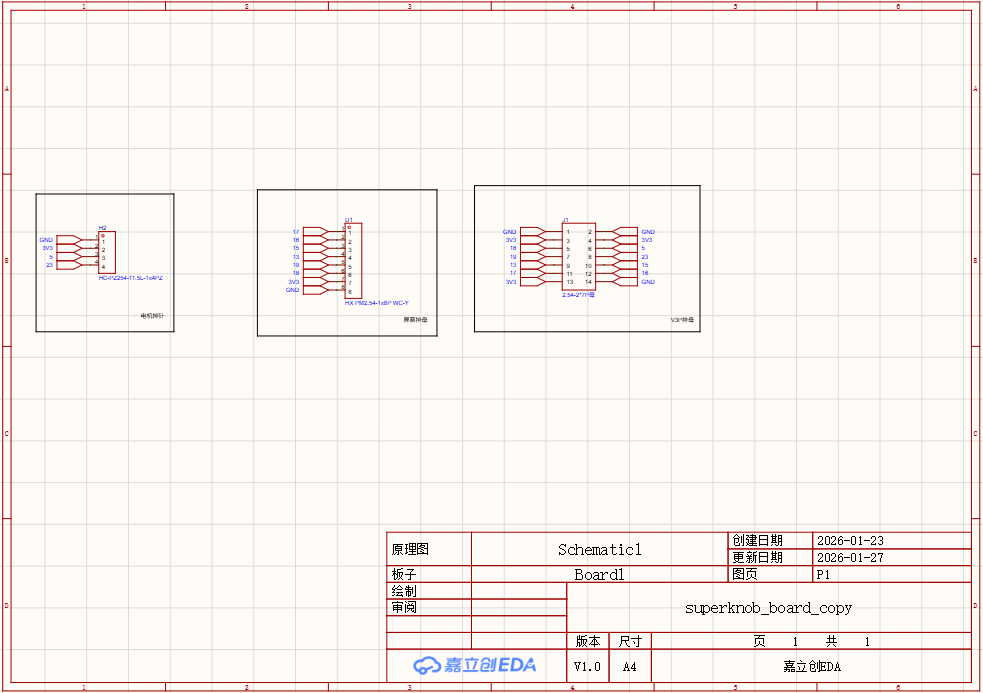
\includegraphics[width=\linewidth]{figures/adapter_display.png}
  \par\small 8 pin 排母接显示屏
\end{minipage}\hfill
\begin{minipage}[b]{0.32\linewidth}
  \centering
  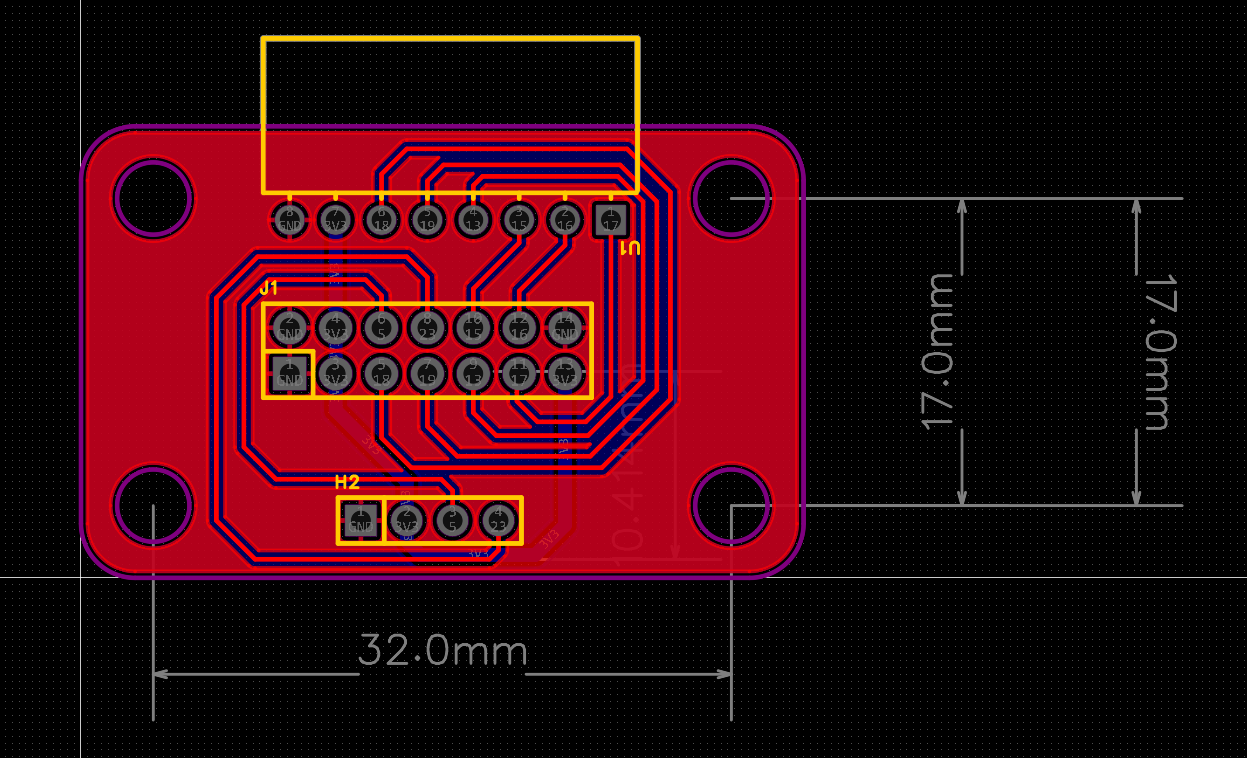
\includegraphics[width=\linewidth]{figures/adapter_driver.png}
  \par\small 排母插接驱动板
\end{minipage}\hfill
\begin{minipage}[b]{0.32\linewidth}
  \centering
  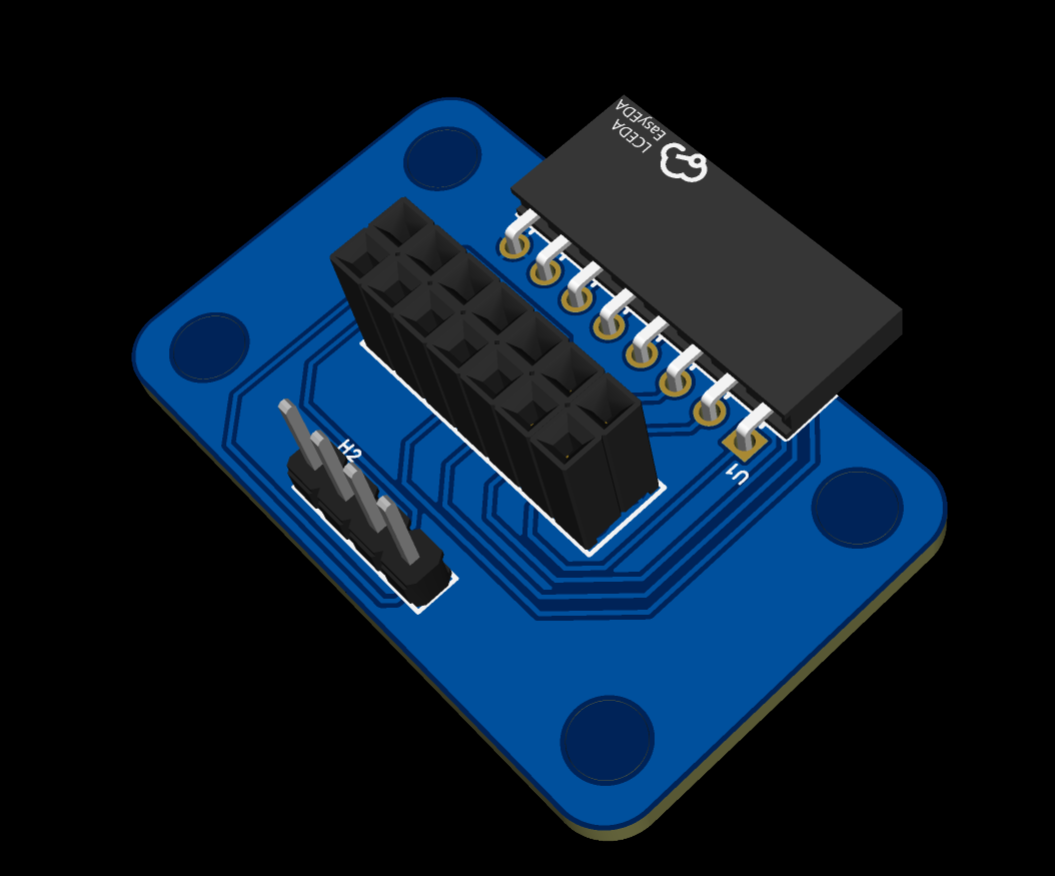
\includegraphics[width=\linewidth]{figures/adapter_encoder.png}
  \par\small 4 pin 排针接编码器 I\textsuperscript{2}C
\end{minipage}
\caption{转接板的显示屏、驱动板与编码器接口}
\label{fig:adapter}
\end{figure}

\subsubsection{外壳建模与装配}

外壳及内部安装结构采用 SolidWorks 建模并以 3D 打印制作，如图 \ref{fig:shell} 所示。建模时按显示屏、电机、转接板、编码器与连接线的实际尺寸确定各安装定位，反复调整以保证结构强度与装配间隙；打印完成后，按磁铁与电机轴同轴、编码器与磁铁间距合适、显示屏固定稳固的要求完成装配。至此，转接板与外壳共同把分散的电气接口和机械零件组织为一个整体，为后续联调提供了稳定可靠的硬件基础。

\begin{figure}[H]
\centering
\begin{minipage}[b]{0.48\linewidth}
  \centering
  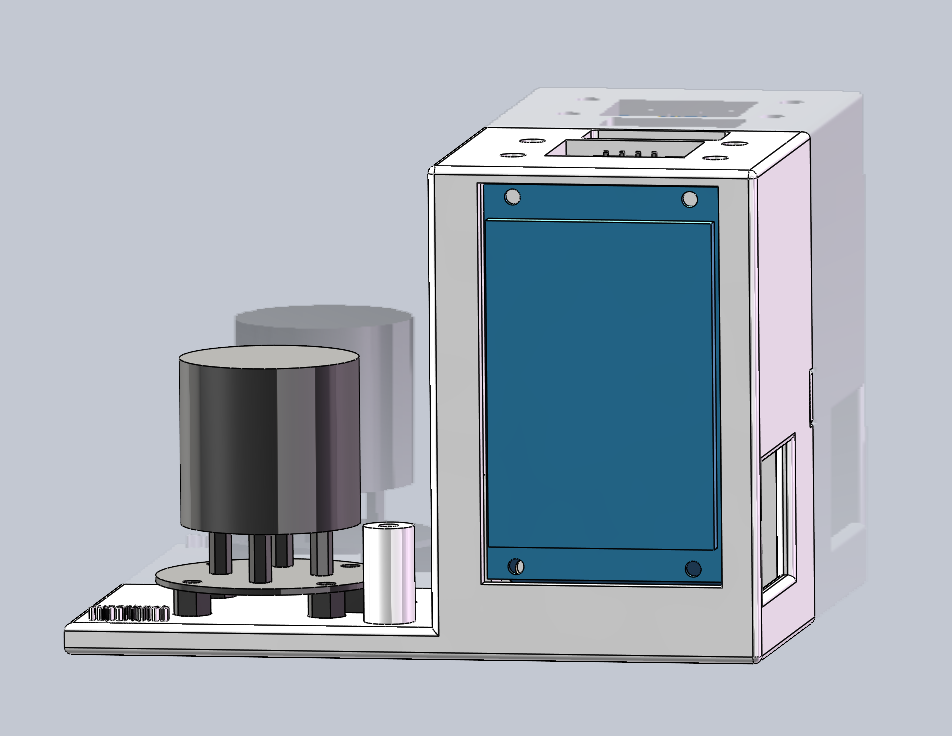
\includegraphics[width=\linewidth]{figures/shell_model_1.png}
\end{minipage}\hfill
\begin{minipage}[b]{0.48\linewidth}
  \centering
  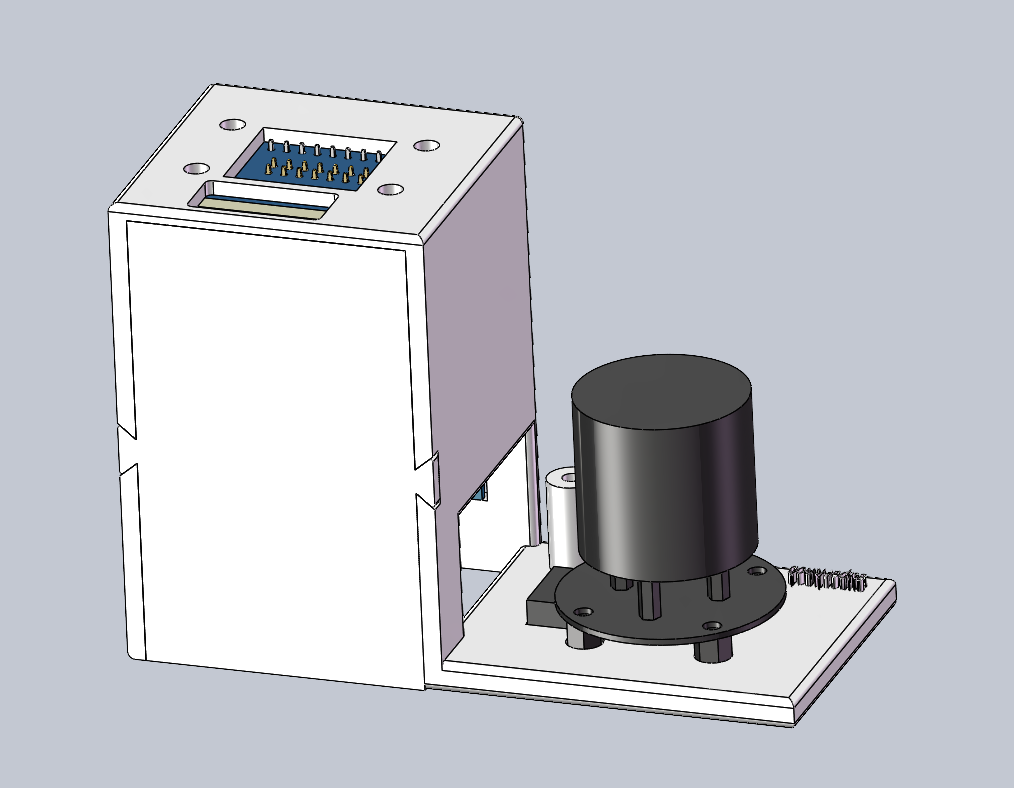
\includegraphics[width=\linewidth]{figures/shell_model_2.png}
\end{minipage}
\caption{SolidWorks 外壳建模}
\label{fig:shell}
\end{figure}

\subsection{软硬件联调过程}

\subsubsection{从编译烧录到屏幕正常显示}

联调开始时，工程还不能稳定完成编译和烧录。我们先在 PlatformIO 中补齐依赖和 LVGL 配置，并解决旧工具链不兼容中文路径的问题。第一次打开串口时输出全是乱码，核对程序后才发现监视器仍使用 9600 baud，而代码设置为 115200 baud；统一波特率后，启动信息终于能够正常阅读。此后每次修改都先确认编译通过，再烧录并查看串口输出，许多问题也因此更容易定位。

屏幕无显示是耗时较长的一次排查。我们先确认背光和供电，再逐项核对屏幕型号、SPI 引脚以及 LVGL 的刷新设置，最后发现实物使用 ST7789，原来的部分配置并不匹配。修改驱动和引脚后，屏幕已经能够点亮，但运行仍不稳定，于是又补充 LVGL 时钟设置，并把显示缓冲改为单个 40 行缓冲，减少内存占用。经过这些调整，页面刷新恢复正常，也为后来加入蓝牙和风扇功能留出了空间。

\subsubsection{触摸、电机与功能页面调试}

触摸键曾出现按一下却连续触发多次的问题。起初我们怀疑 GPIO0 本身受到下载功能影响，尝试把触摸输入改到 GPIO4，但实机现象没有明显改善，因此撤销了这次修改。之后我们改为连续检测到 4 次有效信号才认为按下，并规定手指松开后才能接受下一次输入。电脑控制模式还分别设置按下和松开的阈值，避免数值在临界位置波动。最终单次触摸能够稳定对应一次页面确认或模式切换。

电机不能正常转动时，串口中曾出现 \texttt{Error 263}。查阅并对照运行状态后，我们确认问题来自 AS5600 编码器未被识别，随后重新检查电机独立供电、共地、SDA/SCL 接线和磁铁位置。编码器恢复读数后，再继续调整 FOC 参数和各页面的手感，避免把接线问题误认为控制参数不合适。

风扇功能则按“先读、再写、最后联动页面”的顺序完成。我们先验证 ESP32 能找到风扇并读回型号和状态，再加入开关、风速和左右转动指令。页面接入后发现网络回复会拖慢界面，因此将通信移到单独任务，并合并快速旋转时产生的重复风速请求。随后又处理了中文显示方框、档位到达边界后旋钮难以继续转动等问题。每解决一个问题，都重新烧录并在实机上检查，而不是一次加入全部功能后再集中排错。

表 \ref{tab:debug-loop} 汇总了联调过程中几项较有代表性的问题。

\begin{table}[H]
\centering
\small
\begin{tabular}{p{0.19\linewidth}p{0.26\linewidth}p{0.40\linewidth}}
\toprule
现象 & 定位到的原因 & 处理与验证 \cr
\midrule
工程无法完整链接 & LVGL 配置缺失，旧工具链不兼容中文路径 & 补齐配置并调整工程路径，直到固件能够稳定生成 \cr
屏幕无显示 & 屏幕型号和部分引脚配置与实物不一致 & 改用 ST7789 配置，重新核对 SPI、背光和刷新设置 \cr
触摸重复触发 & 按住时被程序连续识别为多次点击 & 增加连续采样、按下锁定和松开后解锁 \cr
风扇调节时界面卡顿 & 页面需要等待每一次网络回复 & 将联网控制放入单独任务，并合并重复的调速请求 \cr
页面中文显示方框 & 默认字体不包含页面所需汉字 & 根据实际用字重新生成中文字体并检查页面布局 \cr
\bottomrule
\end{tabular}
\caption{主要故障的定位与闭环处理}
\label{tab:debug-loop}
\end{table}

\subsubsection{联调结果}

完成上述调试后，同一套硬件已经能够运行主界面、不同旋钮手感、番茄钟、音乐、两款小游戏、BLE 电脑控制和局域网风扇控制。实机演示中，菜单焦点能随旋钮档位移动，不同页面会切换相应手感；电脑可以收到滚轮、音量、Alt+Tab 和鼠标按键操作，风扇的开关和风速也能随旋钮改变。

项目仍有一些可以继续完善的地方。现有硬件没有相电流采样，手感在负载变化时还不够一致；进入 BLE 模式需要软重启；风扇左右转动的单次角度以及断网后的恢复效果也还需要更多实机测试。这些问题没有影响目前的主要演示，但也让我们认识到，完成页面和控制代码只是第一步，稳定性往往需要在反复烧录、观察和调整中逐渐提高。



\section{项目总结 个人体会与成员分工}

\subsection{项目总结}
\placeholder

\subsection{个人体会}

\subsubsection{李彦霖}

作为项目组长，我参与了项目从方案构想到整机实现的全过程。从零搭建项目架构时，我需要统筹电机控制、LVGL 界面和各功能模块之间的关系，并逐步确定任务划分、通信方式与开发顺序。这一过程使我深入理解了 FOC 的基本原理与触感控制方法，也掌握了利用 FreeRTOS 进行任务调度和跨任务通信的思路。

在开发过程中，我进一步锻炼了软硬件联合调试能力，学会从接线、驱动、控制参数和程序逻辑等多个方面定位问题。同时，组长工作也让我认识到及时沟通和明确分工的重要性。通过与队友协调开发进度、讨论方案并共同解决问题，我在技术实践和团队协作方面都获得了较大提升。

\subsubsection{朱熠正}
\placeholder

\subsubsection{康鑫杰}
\placeholder

\subsection{成员分工}

\begin{table}[H]
\centering
\small
\begin{tabular}{p{0.16\linewidth}p{0.38\linewidth}p{0.33\linewidth}}
\toprule
成员 & 具体分工   \\
\midrule
李彦霖 & FOC 触感引擎实现，LVGL + 电机联调，音乐功能与电机交互展示，跳一跳游戏设计
  \\
朱熠正 & 触摸引脚调试，BLE 电脑控制 + 番茄钟，物联网功能开发
   \\
康鑫杰 & 转接板设计 + 外壳建模，整机装配与集成调试，钓鱼游戏设计
  \\
三人共同工作 & FOC 原理学习、整机联调、稳定性测试、代码整理与结题汇报
  \\
\bottomrule
\end{tabular}
\caption{成员分工记录}
\label{tab:member-division}
\end{table}

\end{document}
